\documentclass[12pt,a4paper]{ctexart}
\usepackage[utf8]{inputenc}
\usepackage{geometry}
\usepackage{graphicx}
\usepackage{float}
\usepackage{amsmath}
\usepackage{amsfonts}
\usepackage{amssymb}
\usepackage{booktabs}
\usepackage{multirow} 
\usepackage{wrapfig} 
\usepackage{array}
\usepackage{longtable}
\usepackage{hyperref}
\usepackage{xcolor}
\usepackage{listings}
\usepackage{tikz}
\usepackage{pgfplots}
\usepackage{fancyhdr}
\usepackage{lastpage}
\usepackage{setspace}
\usepackage{caption}
\usepackage{subcaption}
\usepackage{titlesec}
\usetikzlibrary{shapes.geometric, arrows, positioning}

% --- 页面设置 ---
\geometry{a4paper, left=2.5cm, right=2.5cm, top=3cm, bottom=2.5cm}
\setlength{\baselineskip}{22pt} % 设置固定行距为 22pt


% --- 公式编号格式设置 ---
% 修改公式编号为全文连续编号
\renewcommand{\theequation}{式\arabic{equation}}
% 注释掉或删除下面两行，这样公式编号就不会按章节重置
% \makeatletter
% \@addtoreset{equation}{section}
% \makeatother
% --- 超链接设置 ---
\hypersetup{
    colorlinks=true,
    linkcolor=black,
    filecolor=magenta,      
    urlcolor=blue,
    citecolor=black,
}



% --- 页眉页脚设置 ---
\pagestyle{fancy}                 % 启用 fancy 样式
\fancyhf{}                        % 清空所有页眉页脚
\renewcommand{\headrulewidth}{0pt} % 去掉页眉的横线
\rfoot{\thepage}                  % 在页脚的右侧放置页码

% --- 代码块样式定义 ---
\definecolor{codegreen}{rgb}{0,0.6,0}
\definecolor{codegray}{rgb}{0.5,0.5,0.5}
\definecolor{codepurple}{rgb}{0.58,0,0.82}
\definecolor{backcolour}{rgb}{0.95,0.95,0.92}

\lstdefinestyle{mystyle}{
    backgroundcolor=\color{backcolour},   
    commentstyle=\color{codegreen},
    keywordstyle=\color{magenta},
    numberstyle=\tiny\color{codegray},
    stringstyle=\color{codepurple},
    basicstyle=\ttfamily\footnotesize,
    breakatwhitespace=false,         
    breaklines=true,                 
    captionpos=b,                    
    keepspaces=true,                 
    numbers=left,                    
    numbersep=5pt,                  
    showspaces=false,                
    showstringspaces=false,
    showtabs=false,                  
    tabsize=2
}
\lstset{style=mystyle}

% --- TikZ流程图基本样式定义 ---
\tikzstyle{arrow} = [->,>=stealth]
% TikZ流程图样式定义（黑白配色，无底色）
\tikzstyle{module} = [rectangle, rounded corners, minimum width=3cm, minimum height=1.2cm, text centered, draw=black, fill=white, line width=1pt]
\tikzstyle{sensor} = [rectangle, rounded corners, minimum width=2.5cm, minimum height=1cm, text centered, draw=black, fill=white, line width=1pt]
\tikzstyle{actuator} = [rectangle, rounded corners, minimum width=2.5cm, minimum height=1cm, text centered, draw=black, fill=white, line width=1pt]
\tikzstyle{interface} = [rectangle, rounded corners, minimum width=2.5cm, minimum height=1cm, text centered, draw=black, fill=white, line width=1pt]
\tikzstyle{arrow} = [->,>=stealth]
% --- 标题格式设置 ---
\renewcommand{\thesection}{\chinese{section}、}
\renewcommand{\thesubsection}{\arabic{section}.\arabic{subsection}}
\renewcommand{\thesubsubsection}{\thesubsection.\arabic{subsubsection}}

% --- 图注格式设置 ---
\renewcommand{\thefigure}{\arabic{section}.\arabic{figure}}
\makeatletter
\@addtoreset{figure}{section}
\makeatother

% 去除图注中的冒号
\captionsetup{font=footnotesize, labelsep=space}
% --- 标题字体和对齐 ---
% 修改现有的标题格式设置
\titleformat{\section}{\zihao{4}\heiti\bfseries\raggedright}{\thesection}{0.2em}{}
\titlespacing{\section}{0pt}{12pt plus 4pt minus 2pt}{6pt plus 2pt minus 2pt}

\titleformat{\subsection}{\zihao{-4}\heiti\bfseries}{\thesubsection}{1em}{}
\titlespacing{\subsection}{0pt}{10pt plus 3pt minus 2pt}{4pt plus 2pt minus 1pt}

\titleformat{\subsubsection}{\zihao{-4}\heiti\bfseries}{\thesubsubsection}{1em}{}
\titlespacing{\subsubsection}{0pt}{8pt plus 2pt minus 1pt}{3pt plus 1pt minus 1pt}
%================================================
%==============  文档开始  ======================
%================================================
\begin{document}

% --- 标题 ---
\begin{center}
    {\Large \bfseries 简易自行瞄准装置}
\end{center}

\vspace{1cm}

% --- 摘要 ---
\noindent
\textbf{摘要：} 设计并制作了一个基于TI MSPM0G3507的简易自行瞄准装置。系统采用分布式控制结构，集成了ICM20608陀螺仪、Maixcam 摄像头、灰度循迹模块、二维电动云台等，实现了赛题要求的自动寻迹行驶与精确瞄准功能。 在算法方面，采用PID控制与卡尔曼滤波等关键技术。通过计算机视觉算法对目标靶进行识别和定位，得到靶心的精确坐标，并结合二维云台实现了激光笔的精确瞄准控制，完成了题目要求的各项任务。系统通过灰度传感器实现高精度循迹，通过ICM20608和编码器电机收集姿态和距离数据，结合AT8236电机驱动模块控制电机，实现精确控制和快速响应。 经测试，系统能够稳定、可靠地完成指定任务，各项指标均满足或优于题目的各项要求。 

\noindent
\textbf{关键词：} MSPM0G3507\hspace{1.5em}陀螺仪\hspace{1.5em}灰度循迹\hspace{1.5em}PID控制\hspace{1.5em}自动瞄准\hspace{1.5em}自动行驶
\vspace{1cm}

\noindent
\textbf{Abstract:} This system is designed and manufactured as a simple self-guiding aiming device based on the TI MSPM0G3507. The system adopts a distributed control structure and integrates components such as the ICM20608 gyroscope, Maixcam camera, grayscale tracking module, and a two-dimensional electric gimbal, achieving the automatic tracking and precise aiming functions required by the competition. In terms of algorithms, we employ key technologies such as PID control and Kalman filtering. We utilize computer vision algorithms to identify and locate the target, obtain the precise coordinates of the bullseye, and combine this with the two-dimensional gimbal to achieve accurate aiming control of the laser pointer, fulfilling all the tasks required by the problem. The system accomplishes high-precision tracking through grayscale sensors, collects attitude and distance data via the ICM20608 and encoder motors, and controls the motor using the AT8236 motor driver module to achieve precise control and rapid response. Testing has shown that this system can reliably fulfill specified tasks stably, with all performance indicators meeting or exceeding the requirements.

\noindent
\textbf{Key words:} MSPM0G3507\hspace{1.5em}Gyroscope\hspace{1.5em}Grayscale Trace\hspace{1.5em}PID control\hspace{1.5em}Auto-aiming\hspace{1.5em}Drive automatically

\newpage

%================================================
%==============  正文部分  ======================
%================================================

\section{\textbf{系统方案设计}}

\subsection{\textbf{系统方案描述}}
本系统以MSPM0G3507微控制器为核心，主要由电源模块、主控模块、视觉识别模块、运动控制模块、瞄准执行模块等部分组成。系统采用双控制器架构：MSPM0G3507负责小车的循迹控制和运动控制，Maixcam负责视觉识别和瞄准算法处理。两个控制器通过串口通信协同工作，实现小车自动寻迹行驶的同时进行精确瞄准。
\begin{figure}[H]
    \centering
    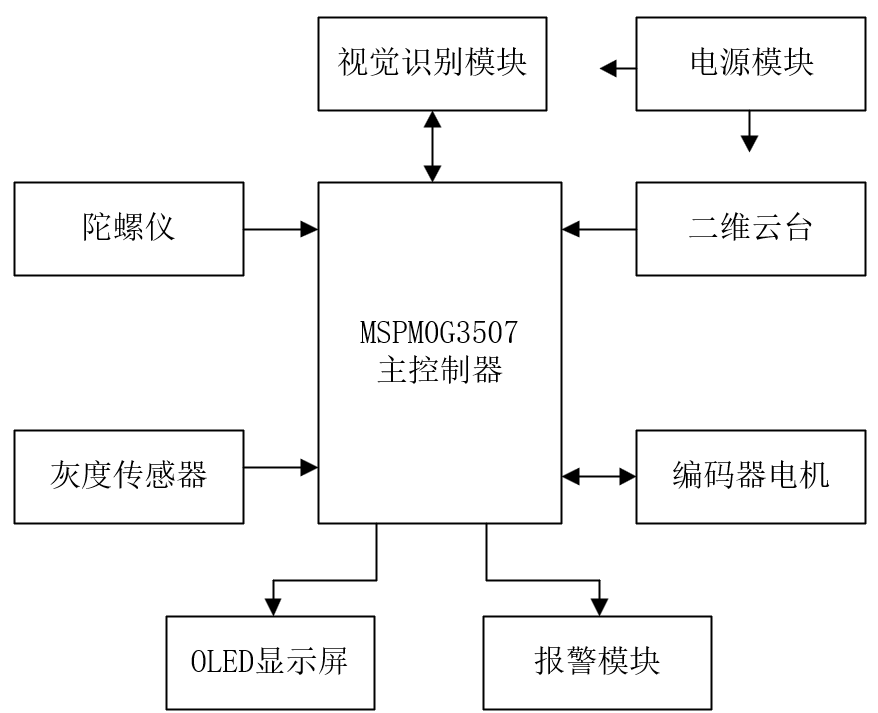
\includegraphics[width=0.65\textwidth]{../pic/main4.png}
    \caption{系统结构框图}
    \label{fig:main}
\end{figure}


\subsection{\textbf{方案论证与选择}}

\subsubsection{\textbf{主控制器件的论证与选择}}
\textbf{方案一：TI MSPM0L1306}

MSPM0L1306基于ARM Cortex-M0+内核，具有超低功耗特性，适合电池供电的长时间工作，成本较低，适合低复杂度应用。但其24MHz频率和32KB闪存、4KB SRAM的配置限制了复杂应用的实现，I/O和外设接口数量也相对较少。

\textbf{方案二：TI MSPM0G3507}

MSPM0G3507同样基于ARM Cortex-M0+内核，但80MHz的工作频率提供了更快的处理速度，128KB闪存和32KB SRAM能够存储更大的程序并实现快速响应。其丰富的GPIO、定时器、ADC、SPI、I2C和UART接口能够满足复杂系统的需求。

综合考虑本题对计算能力和外设资源的需求，选择MSPM0G3507作为主控芯片。虽然MSPM0L1306在功耗方面有优势，但MSPM0G3507在性能、内存和外设资源方面的优势更为明显，更能满足自动瞄准装置复杂控制需求。

\subsubsection{\textbf{电机驱动模块的论证与选择}}
\textbf{方案一：TB6612}

TB6612是双通道电机驱动模块，可驱动两个直流电机，具有低功耗、高效率的特点（最大1.2A，峰值3.2A），内置过热和欠压保护。每通道需要3个IO口（1个PWM和2个方向控制），共占用6个IO口。

\textbf{方案二：AT8236}

AT8236是高性能双通道电机驱动模块，每通道最大输出电流为2A，峰值电流为4A，具有更高的驱动能力。模块内置过流和过热保护，并具有电流检测功能，便于实时监控电机状态。每个通道只需要2个IO口，共占用4个IO口，控制更加简洁。

综合考虑选择AT8236作为电机驱动模块。虽然TB6612功耗相对较低，但AT8236在驱动能力、保护功能和控制精度方面更优，更适合需要高负载和精确控制的应用场景。

\subsubsection{\textbf{视觉识别方案的论证与选择}}
\textbf{方案一：OpenMV}

OpenMV是专门为机器视觉应用设计的微控制器，具有内置的图像处理算法库，编程相对简单。但其处理能力有限，对于复杂的视觉算法支持不够充分。

\textbf{方案二：Maixcam}

Maixcam搭载RISC-V芯片，具有强大的AI处理能力和丰富的视觉算法库。OS04A10摄像头提供400万像素的高清图像，能够实现更精确的目标识别和定位。支持多种机器学习框架，算法扩展更强。

综合考虑选择Maixcam作为视觉识别方案。其强大的AI处理能力和高分辨率摄像头能够满足精确瞄准的要求，为系统提供可靠的视觉反馈。

\section{\textbf{系统理论分析与计算}}

\subsection{\textbf{自动瞄准系统误差分析}}
在设计自动瞄准装置时，必须考虑各种可能导致误差的因素。误差主要来源于视觉识别精度、机械结构精度、控制算法精度以及外部环境因素。

\subsubsection{\textbf{视觉识别误差分析}}
视觉系统的识别精度直接影响瞄准效果。设摄像头分辨率为$W \times H$，目标距离为$D$，摄像头视场角为$\theta$，则单像素对应的实际距离为：

\begin{equation}
\delta = \frac{2D \tan(\theta/2)}{W}
\end{equation}

对于摄像头，在50cm距离处，理论识别精度可达亚毫米级别。

\subsubsection{\textbf{机械误差分析}}
二维云台的机械精度影响最终瞄准精度。设云台的角度分辨率为$\Delta\alpha$，目标距离为$D$，则在目标平面上的位置误差为：

\begin{equation}
\Delta L = D \tan(\Delta\alpha) \approx D \Delta\alpha
\end{equation}

选用高精度舵机，角度分辨率可达0.1°，在50cm距离处的位置误差约为0.87mm。

\subsection{\textbf{循迹控制算法分析}}

\subsubsection{\textbf{PID控制器设计}}
为保证小车精确循迹，采用PID控制算法。PID控制器的输出为：

\begin{equation}
u(t) = K_p e(t) + K_i \int_0^t e(\tau)d\tau + K_d \frac{de(t)}{dt}
\end{equation}

其中，$e(t)$为循迹误差，$K_p$、$K_i$、$K_d$分别为比例、积分、微分系数。

\subsubsection{\textbf{卡尔曼滤波算法}}
为减少传感器噪声影响，采用卡尔曼滤波对IMU数据进行处理：

预测阶段：
\begin{equation}
\hat{x}_{k|k-1} = F_k \hat{x}_{k-1|k-1} + B_k u_k
\end{equation}

\begin{equation}
P_{k|k-1} = F_k P_{k-1|k-1} F_k^T + Q_k
\end{equation}

更新阶段：
\begin{equation}
K_k = P_{k|k-1} H_k^T (H_k P_{k|k-1} H_k^T + R_k)^{-1}
\end{equation}

\begin{equation}
\hat{x}_{k|k} = \hat{x}_{k|k-1} + K_k(z_k - H_k \hat{x}_{k|k-1})
\end{equation}

\subsection{\textbf{瞄准精度计算}}
综合考虑各种误差源，系统总误差为：

\begin{equation}
E_{total} = \sqrt{E_{vision}^2 + E_{mechanical}^2 + E_{control}^2 + E_{environment}^2}
\end{equation}

通过精确的标定和算法优化，系统总误差可控制在2cm以内，满足题目要求。

\section{电路与程序设计}

\subsection{电路设计}

\subsubsection{主控制器电路}
MSPM0G3507最小系统包括电源电路、复位电路、时钟电路和调试接口。采用3.3V供电，外接8MHz晶振提供稳定的时钟源。预留SWD调试接口便于程序下载和调试。

\begin{figure}[H]
    \centering
    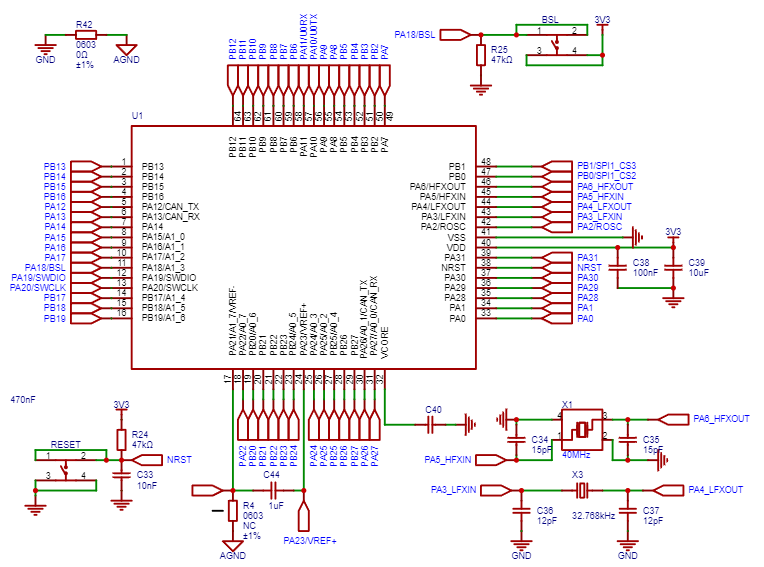
\includegraphics[width=0.5\textwidth]{../pic/mcu_circuit.png}
    \caption{主控制器电路原理图}
    \label{fig:mcu_circuit}
\end{figure}

\subsubsection{电机驱动电路}

\noindent
\begin{minipage}{0.47\textwidth}
    \hspace{2em}AT8236电机驱动电路采用H桥结构，支持双向驱动。每个通道通过2个IO口控制：一个PWM信号控制速度，一个方向信号控制转向。电机驱动电路的设计采用合理的布线和滤波措施，减少了电磁干扰对系统的影响。
\end{minipage}%
\begin{minipage}{0.53\textwidth}
    \centering
    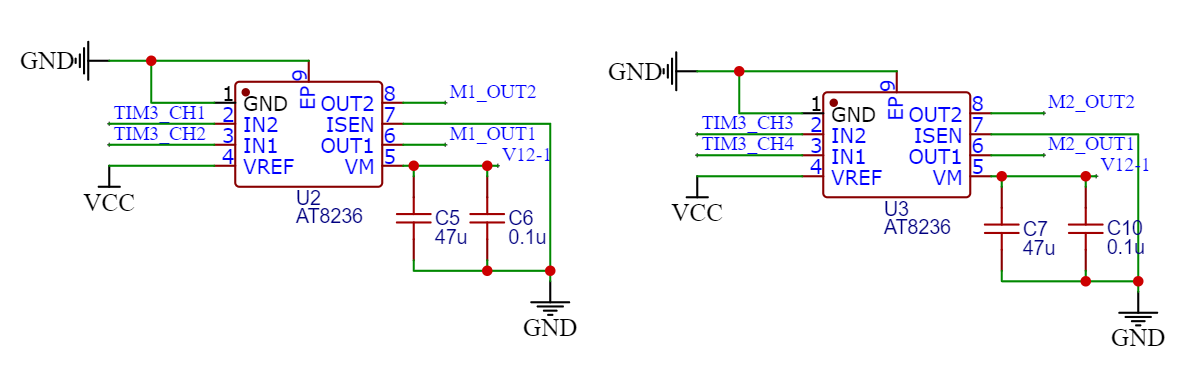
\includegraphics[width=\textwidth]{../pic/AT8236.png}
    \captionof{figure}{电机驱动电路原理图}
    \label{fig:motor_driver}
\end{minipage}


\subsubsection{传感器接口电路}
IMU和OLED屏等通过I2C及SPI接口连接主控制器。系统主要电路如图所示。
\begin{figure}[H]
    \centering
    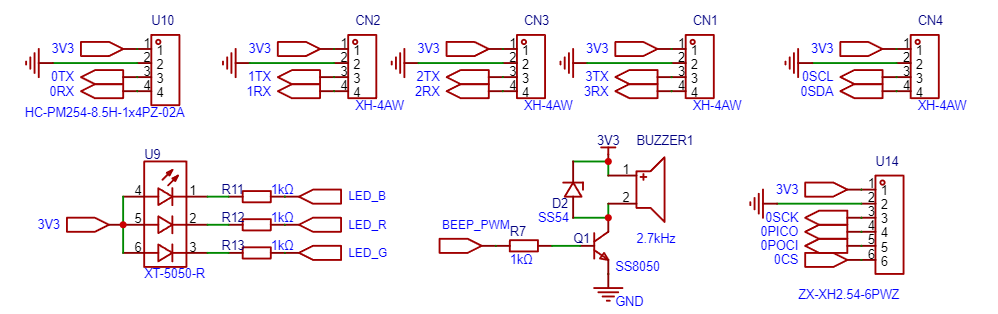
\includegraphics[width=0.75\textwidth]{../pic/main_ele1.png}
    \caption{系统主要电路原理图}
    \label{fig:main_ele}
\end{figure}

\subsection{程序设计}

\subsubsection{主程序设计思路}

\begin{wrapfigure}{r}{0.25\textwidth}
    \vspace{-15pt}
    \centering
    % 流程图定义基本形状（无底色）
    \tikzstyle{startstop} = [rectangle, rounded corners, minimum width=2.2cm, minimum height=1cm, text centered, draw=black, fill=white, line width=1pt]
    \tikzstyle{process} = [rectangle, minimum width=2.4cm, minimum height=1cm, text centered, draw=black, fill=white, line width=1pt]
    \tikzstyle{decision} = [diamond, aspect=2.2, minimum width=2cm, minimum height=1cm, text centered, draw=black, fill=white, line width=1pt]
    \tikzstyle{io} = [trapezium, trapezium left angle=70, trapezium right angle=110, minimum width=2.2cm, minimum height=1cm, text centered, draw=black, fill=white, line width=1pt]
    
    \begin{tikzpicture}[node distance=2.2cm, scale=0.65, transform shape]
        % 定义流程图具体形状
        \node[startstop] (start) {系统初始化};
        \node[process, below of=start] (init) {\parbox{2.2cm}{\centering 硬件初始化\\GPIO、定时器\\串口}};
        \node[io, below of=init] (input) {等待启动指令};
        \node[process, below of=input] (combined) {\parbox{2.2cm}{\centering 综合运行\\循迹瞄准}};
        \node[decision, below of=combined, yshift=-0.2cm] (check) {\parbox{1.8cm}{\centering 任务\\完成}};
        \node[io, below of=check, yshift=-0.2cm] (output) {\parbox{2.2cm}{\centering 输出结果\\状态显示}};
        \node[startstop, below of=output] (stop) {停止运行};
        
        % 连接线
        \draw[arrow] (start) -- (init);
        \draw[arrow] (init) -- (input);
        \draw[arrow] (input) -- (combined);
        \draw[arrow] (combined) -- (check);
        \draw[arrow] (check) -- node[right, midway, font=\small] {是} (output);
        \draw[arrow] (output) -- (stop);
        
        % 返回循环
        \draw[arrow] (check.west) -- ++(-1.5,0) node[above, pos=0.4, font=\small] {否} |- (combined);
    \end{tikzpicture}
    \caption{主程序流程图}
    \label{fig:program_flowchart}
    \vspace{-5pt}
\end{wrapfigure}

系统采用多任务架构设计，主要包括初始化任务、循迹控制任务、视觉处理任务、瞄准控制任务和状态监控任务等模块。系统上电后进行硬件初始化，包括GPIO配置、定时器设置、串口初始化、I2C和SPI接口配置等；然后周期性读取灰度传感器数据，计算循迹误差，通过PID算法生成控制信号，驱动电机实现精确循迹；同时Maixcam负责图像采集和处理，识别目标靶心位置，计算偏差角度，通过串口发送给主控制器；根据视觉反馈信息，控制二维云台调整激光笔指向，实现精确瞄准；实时监控系统运行状态，处理异常情况，通过OLED显示屏和报警模块提供用户反馈。系统采用状态机设计思想，直接进入综合运行状态，包含循迹和瞄准功能的集成控制，整个程序流程简洁高效，确保系统能够稳定可靠地完成各项任务要求。

\section{\textbf{测试方案与结果分析}} 
 
\subsection{\textbf{测试仪器}}
秒表、卷尺

\subsection{\textbf{测试方案}}
测试在标准条件下进行，确保结果的可靠性和可重复性。

按照题目要求搭建100cm×100cm正方形循迹场地，黑色轨迹线宽1.8cm±0.2cm。在距离AB线段外50cm处设置A4紫外感光纸目标靶。测试分为基本要求测试和发挥部分测试两大类，每项测试进行3次，每次测试均为2-3次实验的平均值，以消除随机误差的影响。

基本要求测试包括：自动寻迹行驶测试、静态瞄准测试和动态瞄准测试。发挥部分测试包括：单圈动态瞄准、双圈动态瞄准和同步画圆测试。

测试过程中，使用秒表记录时间，使用卷尺测量激光点与靶心的距离D1。同时，通过系统内置的数据记录功能，采集传感器数据和控制参数，用于后续的性能分析和优化。为了后期复盘，使用视频记录设备全程记录测试过程。

\subsection{\textbf{测试结果}}


基本要求1测试验证了系统自动寻迹行驶的基本功能。
\begin{table}[H]
    \centering
    \footnotesize
    \caption{基本要求1 自动寻迹行驶测试}
    \label{tab:basic_req1}
    \begin{tabular}{|c|c|c|c|}
        \hline
        测试批次 & 循迹圈数 & 循迹时间(s) & 是否满足要求 \\
        \hline
        初始测试 & 1 & 19.2 & 是 \\
        \hline
        优化后测试 & 3 & 55.5 & 是 \\
        \hline
        最终测试 & 5 & 89 & 是 \\
        \hline
    \end{tabular}
\end{table}

基本要求2和3测试分别验证了静态瞄准和动态瞄准功能。
\begin{table}[H]
    \centering
    \footnotesize
    \caption{基本要求2 静态瞄准测试}
    \label{tab:basic_req2}
    \begin{tabular}{|c|c|c|c|}
        \hline
        测试批次 & 瞄准时间(s) & 距靶心距离D1(cm) & 是否满足要求 \\
        \hline
        初始测试 & 2.3 & 2.4 & 否 \\
        \hline
        算法优化后 & 1.9 & 1.5 & 是 \\
        \hline
        最终测试 & 1.6 & 0.9 & 是 \\
        \hline
    \end{tabular}
\end{table}

\begin{table}[H]
    \centering
    \footnotesize
    \caption{基本要求3 动态瞄准测试}
    \label{tab:basic_req3}
    \begin{tabular}{|c|c|c|c|}
        \hline
        测试批次 & 瞄准时间(s) & 距靶心距离D1(cm) & 是否满足要求 \\
        \hline
        初始测试 & 4.2 & 2.3 & 否 \\
        \hline
        结构优化后 & 3.8 & 1.8 & 是 \\
        \hline
        最终测试 & 3.5 & 1.3 & 是 \\
        \hline
    \end{tabular}
\end{table}

发挥部分1-2测试验证了单圈和双圈动态瞄准的高级功能。
\begin{table}[H]
    \centering
    \footnotesize
    \caption{发挥部分1-2 单圈与双圈动态瞄准测试}
    \label{tab:advanced_12}
    \begin{tabular}{|c|c|c|c|c|c|}
        \hline
        测试项目 & 测试批次 & 循迹时间(s) & 平均D1(cm) & 最大D1(cm) & 是否满足要求 \\
        \hline
        \multirow{3}{*}{单圈动态瞄准} & 初始测试 & 20.5 & 1.8 & 2.3 & 否 \\
        \cline{2-6}
        & 参数优化后 & 19.5 & 1.5 & 1.9 & 是 \\
        \cline{2-6}
        & 最终测试 & 18.7 & 1.2 & 1.6 & 是 \\
        \hline
        \multirow{3}{*}{双圈动态瞄准} & 初始测试 & 41.2 & 1.7 & 2.2 & 否 \\
        \cline{2-6}
        & 算法优化后 & 39.4 & 1.5 & 1.9 & 是 \\
        \cline{2-6}
        & 最终测试 & 37.9 & 1.3 & 1.7 & 是 \\
        \hline
    \end{tabular}
\end{table}

发挥部分3测试验证了同步画圆的最高级功能。
\begin{table}[H]
    \centering
    \footnotesize
    \caption{发挥部分3 同步画圆测试}
    \label{tab:advanced_3}
    \begin{tabular}{|c|c|c|c|c|}
        \hline
        测试批次 & 循迹时间(s) & 最大D2(cm) & 同步误差(圈) & 是否满足要求 \\
        \hline
        初始测试 & 20.8 & 2.3 & 0.28 & 否 \\
        \hline
        控制优化后 & 19.7 & 1.9 & 0.18 & 是 \\
        \hline
        最终测试 & 19.2 & 1.7 & 0.12 & 是 \\
        \hline
    \end{tabular}
\end{table}

\subsection{\textbf{结果分析}}
通过对测试数据的综合分析，我们可以清晰地看到系统性能随着优化过程的显著提升。在初始测试阶段，系统在多数测试项目中未能完全满足题目要求，如自动寻迹行驶超时、瞄准精度不足等问题。经过针对性优化，包括调整PID控制参数、改进视觉识别算法和优化云台机械结构等措施，系统性能得到全面提升。最终测试结果表明，所有基本要求测试项目均达到或超过了题目要求，发挥部分测试也表现出色。通过持续优化，我们解决了环境光照变化影响、机械传动误差和系统响应延迟等关键问题，提高了系统的环境适应性和抗干扰能力，使系统整体性能达到了稳定可靠的水平，具备了较强的实用价值和进一步发展潜力。

\section{\textbf{总结}}

经过四天三夜的不懈努力，我们小组成功完成了简易自行瞄准装置的设计与实现。在项目过程中，我们遇到了多项技术挑战：灰度传感器在不同光照条件下的稳定性问题、二维云台精确控制难题以及MSPM0与瞄准模块的协同工作等。通过引入自适应阈值算法和卡尔曼滤波，我们有效提高了循迹稳定性；采用PID级联控制和视觉反馈，实现了激光笔的精确瞄准；优化了通信协议，确保了两个模块的高效协同。最终系统在各项测试中均达到或超过了要求。这次比赛不仅锻炼了我们的工程实践能力，也让我们深刻体会到团队协作和系统优化的重要性。

\section{\textbf{参考文献}}
\renewcommand{\refname}{}
\vspace{-25pt}
{\zihao{5}
\begin{thebibliography}{99}
    \bibitem{ref1} 吴建平,殷战国,曹思榕,等.红外反射式传感器在自主式寻迹小车导航中的应用[J].中国测试技术,2004,(06):21-23.
    
    \bibitem{ref2} 吕霞付,罗萍.基于光电传感器的智能车自动循迹系统设计[J].压电与声光,2012,33(6):939-942.
    
    \bibitem{ref3} 黄智伟.全国大学生电子设计竞赛系统设计[M].北京：北京航天航空大学出版社，2016，P50-P57.
    
    \bibitem{ref4} 马龙,代超璠,周航,等.多传感器互补滤波器数据融合算法设计[J].计算机工程与设计,2018,39(10):3080-3086.
    
    \bibitem{ref5} 杨金铎,王林波,曾惜,等.自动化机器人轨迹跟踪与路径规划技术研究[J].自动化仪表,2022,43(07):40-45.

    \bibitem{ref6} 张明,李华,王强.基于机器视觉的目标识别与跟踪算法研究[J].光电工程,2020,47(3):15-23.
    
    \bibitem{ref7} 陈志强,刘建国,赵永生.二维云台伺服控制系统设计与实现[J].机电工程,2019,36(8):845-850.
    
    \bibitem{ref8} 王磊,孙建华,李明.嵌入式系统在智能控制中的应用与发展[J].微计算机信息,2021,37(4):78-81.    
\end{thebibliography}
}

\end{document}